% Part XII: Complete F* Formalization
% This is a FRAGMENT - no \documentclass, \begin{document}, or \end{document}

\part{Complete F* Formalization}
\label{part:fstar-formalization}

%%%%%%%%%%%%%%%%%%%%%%%%%%%%%%%%%%%%%%%%%%%%%%%%%%%%%%%%%%%%%%%%%%%%%%%%%%%%%%%
\chapter{Module Structure}
\label{chap:module-structure}
%%%%%%%%%%%%%%%%%%%%%%%%%%%%%%%%%%%%%%%%%%%%%%%%%%%%%%%%%%%%%%%%%%%%%%%%%%%%%%%

\begin{fstarcode}[title={Brrr-Machine F* Module Structure}]
(* =======================================================================
   BRRR-MACHINE F* MODULE STRUCTURE
   ======================================================================= *)
(*
  BrrrMachine
  +-- Core
  |   +-- AbstractDomain      -- Lattices, Galois connections
  |   +-- Domains             -- Concrete domains (intervals, taint, etc.)
  |   +-- Effects             -- Effect types and rows
  |   +-- Ownership           -- Resource algebras, ownership states
  |
  +-- Representation
  |   +-- IR                  -- Intermediate representation
  |   +-- CPG                 -- Code Property Graph types
  |   +-- CPG.Builder         -- CPG construction
  |   +-- CPG.Traversal       -- Graph traversal primitives
  |
  +-- Analysis
  |   +-- IFDS                -- IFDS algorithm
  |   +-- PointerAnalysis     -- Andersen, Steensgaard
  |   +-- TaintAnalysis       -- Source-sink analysis
  |   +-- NullAnalysis        -- Nullability tracking
  |   +-- ResourceAnalysis    -- Lifecycle tracking
  |   +-- OwnershipAnalysis   -- Rust-style ownership
  |   +-- RaceDetection       -- Data race detection
  |
  +-- Security
  |   +-- Taint               -- Taint sources, sinks, sanitizers
  |   +-- Vulnerabilities     -- Vulnerability types
  |   +-- SARIF               -- Output format
  |
  +-- Boundary
  |   +-- Languages           -- Language configurations
  |   +-- Boundaries          -- Boundary detection and analysis
  |   +-- Risks               -- Risk calculation
  |
  +-- Incremental
  |   +-- Thunks              -- Cached computations
  |   +-- IncrementalCPG      -- Incremental graph
  |
  +-- Theorems
      +-- Soundness           -- Soundness proofs
      +-- Termination         -- Termination proofs
      +-- Correctness         -- Correctness lemmas
*)
\end{fstarcode}

%%%%%%%%%%%%%%%%%%%%%%%%%%%%%%%%%%%%%%%%%%%%%%%%%%%%%%%%%%%%%%%%%%%%%%%%%%%%%%%
\chapter{Key Soundness Theorems}
\label{chap:soundness-theorems}
%%%%%%%%%%%%%%%%%%%%%%%%%%%%%%%%%%%%%%%%%%%%%%%%%%%%%%%%%%%%%%%%%%%%%%%%%%%%%%%

\begin{pillarbox}[title={Foundational References}]
\begin{itemize}
\item \textbf{[Cousot77]} --- Abstract Interpretation Soundness
\item \textbf{[Reps95]} --- IFDS Algorithm Soundness and Completeness
\item \textbf{[HerlihyWing90]} --- Linearizability and Locality Theorem
\item \textbf{[SabelfeldMyers03]} --- Information Flow Soundness
\item \textbf{[Zilberstein23]} --- Outcome Logic Theorems
\item \textbf{[Bruni23]} --- Local Completeness
\end{itemize}
\end{pillarbox}

\begin{fstarcode}[title={Soundness Theorems Module}]
module BrrrMachine.Theorems.Soundness

(* --------------------------------------------------
   ABSTRACT INTERPRETATION SOUNDNESS
   Source: Cousot 1977
   -------------------------------------------------- *)
(* If abstract analysis says "safe", concrete execution is safe *)
val abstract_interpretation_sound :
  #c:Type -> #a:Type ->
  gc:galois_connection c a ->
  transfer_concrete:(c -> c) ->
  transfer_abstract:(a -> a) ->
  (* Transfer function is sound *)
  (forall x. gc.alpha (transfer_concrete x) `leq`
             transfer_abstract (gc.alpha x)) ->
  (* Fixpoint is sound *)
  Lemma (gc.alpha (lfp transfer_concrete) `leq`
         compute_fixpoint transfer_abstract)
\end{fstarcode}

\begin{theorem}[IFDS Soundness --- \textbf{[Reps95]}]
The IFDS solution is sound: all reported facts actually hold.
\begin{fstarcode}[title={IFDS Soundness}]
val ifds_sound :
  #d:Type ->
  problem:ifds_problem d ->
  node:node_id ->
  fact:d ->
  (* If fact is in the solution *)
  (node, fact) `mem` solve problem ->
  (* Then there exists a concrete execution where fact holds *)
  Lemma (exists exec. reaches exec node /\ fact_holds exec node fact)
\end{fstarcode}
\end{theorem}

\begin{theorem}[IFDS Completeness for Distributive Problems]
For distributive dataflow problems, IFDS is complete.
\begin{fstarcode}[title={IFDS Completeness}]
val ifds_complete :
  #d:Type ->
  problem:ifds_problem d ->
  (* Problem is distributive *)
  (forall e s1 s2. problem.transfer e (s1 `union` s2) ==
                   problem.transfer e s1 `union` problem.transfer e s2) ->
  node:node_id ->
  fact:d ->
  (* If fact actually holds in some execution *)
  (exists exec. reaches exec node /\ fact_holds exec node fact) ->
  (* Then it's in the solution *)
  Lemma ((node, fact) `mem` solve problem)
\end{fstarcode}
\end{theorem}

\begin{fstarcode}[title={Taint Analysis Soundness}]
(* No false negatives: all actual taint flows are detected *)
val taint_analysis_sound :
  cpg:cpg ->
  sources:(node_id -> option taint_source) ->
  sinks:(node_id -> option taint_sink) ->
  sanitizers:(node_id -> option sanitizer) ->
  result:taint_analysis_result ->
  (* Result is from our analysis *)
  result == run_taint_analysis cpg sources sinks sanitizers ->
  (* For any concrete execution *)
  forall (exec : concrete_execution).
    (* If tainted data reaches a sink unsanitized *)
    (exists src sink. is_source src /\ is_sink sink /\
     reaches_unsanitized exec src sink) ->
    (* Then we reported it *)
    Lemma (exists flow. flow `mem` result.flows /\
           flow.source_location == src /\ flow.sink_location == sink)
\end{fstarcode}

\begin{theorem}[Locality Theorem --- \textbf{[HerlihyWing90]}]
Linearizability is compositional.
\begin{fstarcode}[title={Locality Theorem}]
val locality_theorem :
  h:history ->
  specs:(string -> sequential_spec) ->
  Lemma (linearizable h (combined_spec specs) <==>
         (forall obj. linearizable (subhistory h obj) (specs obj)))
\end{fstarcode}
\end{theorem}

\begin{fstarcode}[title={Information Flow and Outcome Logic}]
(* If implicit flow analysis reports no leaks, noninterference holds *)
val implicit_analysis_sound :
  cpg -> labeling:(string -> security_level) ->
  (run_implicit_analysis cpg labeling = []) ->
  Lemma (termination_insensitive_noninterference (semantics cpg) labeling)

(* Falsification completeness: if spec is violated, we can prove it *)
val falsification_complete :
  pre:outcome_assertion -> prog:program -> post:outcome_assertion ->
  Lemma (requires (not (valid_ol_triple pre prog post)))
        (ensures (valid_ol_triple pre prog (OAConj (OANot post) OATop)))

(* If locally complete, abstract analysis is EXACT for that input *)
val local_completeness_precision :
  #a:Type ->
  dom:abstract_domain a ->
  f:(concrete -> concrete) ->
  f_sharp:(a -> a) ->
  c:concrete ->
  is_locally_complete dom f c ->
  (forall x. dom.lat.alpha (f x) `leq` f_sharp (dom.lat.alpha x)) ->
  Lemma (dom.lat.alpha (f c) = f_sharp (dom.lat.alpha c))
\end{fstarcode}

%%%%%%%%%%%%%%%%%%%%%%%%%%%%%%%%%%%%%%%%%%%%%%%%%%%%%%%%%%%%%%%%%%%%%%%%%%%%%%%
\chapter{Provable Bug Classification (Manifest/Latent)}
\label{chap:manifest-latent}
%%%%%%%%%%%%%%%%%%%%%%%%%%%%%%%%%%%%%%%%%%%%%%%%%%%%%%%%%%%%%%%%%%%%%%%%%%%%%%%

\begin{pillarbox}[title={Replacing Heuristics with Provable Classification}]
\textbf{Source}: \textbf{[Le22]} (ISL) via \textbf{[Vanegue25]} --- ``Non-Termination Proving''

\textbf{OLD (HEURISTIC)}: confidence = 0.0 to 1.0 float\\
\emph{Problem}: No formal semantics. What does ``0.7 confidence'' mean?

\textbf{NEW (PROVABLE)}: Manifest vs Latent classification
\begin{itemize}
\item \textbf{Manifest}: Bug triggers IN ALL CALLING CONTEXTS
\item \textbf{Latent}: Bug triggers ONLY IN SPECIFIC CONTEXTS
\end{itemize}

\textbf{KEY THEOREM (True Positives Property)}:\\
Manifest bugs are GUARANTEED to be real bugs (no false positives).\\
This is a THEOREM, not a heuristic!
\end{pillarbox}

\begin{definition}[ISL Triple --- \textbf{[Le22]}]
An Incorrectness Separation Logic Triple $[p]\, C\, [q; \mathit{exit}]$ consists of:
\begin{itemize}
\item $p$ = PRESUMPTION (existentially quantified precondition)
\item $C$ = CODE
\item $q$ = RESULT (postcondition)
\item $\mathit{exit}$ = EXIT CONDITION ($\mathsf{Ok}$ or $\mathsf{Er}$ for error)
\end{itemize}
\textbf{Semantics}: If $C$ starts in state satisfying $p$ and terminates with exit condition, then result satisfies $q$.
\end{definition}

\begin{fstarcode}[title={ISL Triple and Manifest/Latent Classification}]
module BrrrMachine.ManifestLatent

type exit_condition = Ok | Er  (* Normal vs Error termination *)

type isl_triple = {
  presumption : assertion;      (* p - starting states (existential) *)
  code : cpg_slice;             (* C - analyzed code *)
  result : assertion;           (* q - ending states *)
  exit_cond : exit_condition;   (* Ok or Er *)
}

(* --------------------------------------------------
   MANIFEST vs LATENT CLASSIFICATION (Le 2022, Definition 3.3)
   A bug is MANIFEST if it satisfies ALL of these conditions:
   1. Exit condition is Er (error)
   2. Presumption is emp /\ true (empty heap, no constraints)
   3. Result assertion is satisfiable
   4. All heap locations in result are existentially quantified
   5. Pure constraints in result are universally satisfiable

   MANIFEST = Bug triggers regardless of calling context
   LATENT = Bug requires specific calling context to trigger
   -------------------------------------------------- *)
type bug_classification =
  | Manifest : proof:manifest_proof -> bug_classification
  | Latent : required_context:assertion -> bug_classification
  | RelaxedManifest : violations:list manifest_violation -> bug_classification

type manifest_proof = {
  triple : isl_triple;
  empty_pre : squash (triple.presumption `equiv` (emp `conj` true_pure));
  result_sat : squash (satisfiable triple.result);
  locs_existential : squash (locs (spatial triple.result) `subset`
                             existential_vars triple.result);
  pure_universal : squash (forall_instantiations_sat (pure triple.result));
}
\end{fstarcode}

\begin{theorem}[True Positives Property --- \textbf{[Le22]}, Theorem 3.4]
If a bug is classified as MANIFEST, then either:
\begin{enumerate}
\item[(a)] The code is dead (unreachable), OR
\item[(b)] There EXISTS a concrete input that triggers the bug
\end{enumerate}
This is the fundamental soundness theorem for bug detection. It guarantees NO FALSE POSITIVES for manifest bugs.

\begin{fstarcode}[title={True Positives Property}]
val true_positives_property :
  cpg:cpg -> triple:isl_triple -> proof:manifest_proof ->
  Lemma (is_dead_code cpg triple.code \/
         (exists input. triggers_bug cpg input triple))
\end{fstarcode}
\end{theorem}

\begin{theorem}[Falsification Completeness --- \textbf{[Le22]}, Theorem 3.5]
If a bug is LATENT with required context $C$, then ANY calling context satisfying $C$ will trigger the bug.

\begin{fstarcode}[title={Falsification Completeness}]
val falsification_completeness :
  cpg:cpg -> triple:isl_triple -> required_ctx:assertion ->
  Latent? (classify_bug triple) ->
  classify_bug triple = Latent required_ctx ->
  Lemma (forall ctx_state. ctx_state `satisfies` required_ctx ==>
         triggers_bug cpg ctx_state triple)
\end{fstarcode}
\end{theorem}

\begin{definition}[Relaxed Manifest Criterion --- \textbf{[Le22]} Section 4]
Strict manifest requires $\mathsf{emp}$ precondition (empty heap). RELAXED allows non-emp precondition IF:
\begin{itemize}
\item All heap cells in precondition are POSITIVE (allocated, not deallocated)
\item No negative cells (freed memory) in precondition
\end{itemize}
A heap cell is ``positive'' if it represents allocated memory ($x \mapsto v$), not deallocated memory or an absence constraint.
\end{definition}

\begin{fstarcode}[title={ISL Consequence Rule}]
(* --------------------------------------------------
   ISL CONSEQUENCE RULE (Le 2022)
   NOTE: Entailment direction is REVERSED from Hoare logic!

   Hoare: p' |= p, {p} C {q}, q |= q'  ==>  {p'} C {q'}
   ISL:   p |= p', [p] C [q], q |= q'  ==>  [p'] C [q']
          ^^^^^^
          WEAKENED precondition entails ORIGINAL (opposite direction!)

   REASON: ISL is under-approximate. Weaker precondition means FEWER
   starting states, which is sound for "bug exists" claims.
   -------------------------------------------------- *)
val isl_consequence :
  triple:isl_triple ->
  p':assertion{p' |= triple.presumption} ->  (* p' entails p *)
  q':assertion{triple.result |= q'} ->       (* q entails q' *)
  isl_triple
\end{fstarcode}

%%%%%%%%%%%%%%%%%%%%%%%%%%%%%%%%%%%%%%%%%%%%%%%%%%%%%%%%%%%%%%%%%%%%%%%%%%%%%%%
\section{Occurrence Typing Soundness Theorems}
\label{sec:occurrence-typing-soundness}
%%%%%%%%%%%%%%%%%%%%%%%%%%%%%%%%%%%%%%%%%%%%%%%%%%%%%%%%%%%%%%%%%%%%%%%%%%%%%%%

\begin{pillarbox}[title={Occurrence Typing Soundness --- \textbf{[TobinHochstadt08]}}]
The key theorem: Type refinements are SOUND with respect to runtime values.

If occurrence typing says variable $x$ has type $\tau$ at program point $p$, then at runtime, the value of $x$ is indeed a member of $\tau$.

\textbf{CRITICAL INSIGHT}: Soundness requires VISIBLE predicates to be accurate. A visible predicate can only be established by an ACTUAL runtime check.
\end{pillarbox}

\begin{fstarcode}[title={Occurrence Typing Soundness}]
module BrrrMachine.Theorems.OccurrenceTyping

(* A visible predicate is a proposition known to hold at the current point *)
type visible_predicate =
  | VPHasType : var:string -> ty:ir_type -> visible_predicate
  | VPNotType : var:string -> ty:ir_type -> visible_predicate
  | VPAnd : visible_predicate -> visible_predicate -> visible_predicate
  | VPOr : visible_predicate -> visible_predicate -> visible_predicate
  | VPTrue : visible_predicate
  | VPFalse : visible_predicate

(* Restrict operation: narrow sigma to tau *)
val restrict : ir_type -> ir_type -> ir_type
let rec restrict sigma tau =
  match sigma with
  | TUnion types ->
      let filtered = List.filter (fun t -> types_overlap t tau) types in
      type_union_of_list filtered
  | TTop -> tau
  | _ ->
      if subtype sigma tau then sigma
      else if subtype tau sigma then tau
      else TBottom  (* No overlap *)

(* THEOREM: restrict is sound *)
val restrict_sound :
  sigma:ir_type -> tau:ir_type ->
  v:runtime_value ->
  Lemma (requires value_has_type v sigma && value_has_type v tau)
        (ensures value_has_type v (restrict sigma tau))
\end{fstarcode}

%%%%%%%%%%%%%%%%%%%%%%%%%%%%%%%%%%%%%%%%%%%%%%%%%%%%%%%%%%%%%%%%%%%%%%%%%%%%%%%
\chapter{Under-Approximation Theorems}
\label{chap:under-approximation}
%%%%%%%%%%%%%%%%%%%%%%%%%%%%%%%%%%%%%%%%%%%%%%%%%%%%%%%%%%%%%%%%%%%%%%%%%%%%%%%

\begin{pillarbox}[title={Dual Soundness: Over-Approximation vs Under-Approximation}]
\textbf{VERIFICATION SOUNDNESS (over-approx)}: $\alpha(\text{concrete}) \subseteq \text{abstract}$\\
``If analysis says safe, truly safe'' --- may have FALSE POSITIVES

\textbf{DETECTION SOUNDNESS (under-approx)}: $\text{abstract} \subseteq \text{concrete}$\\
``If analysis says bug, truly a bug'' --- may have FALSE NEGATIVES

The synthesis REQUIRES BOTH for complete analysis.
\end{pillarbox}

\begin{fstarcode}[title={Under-Approximation Theorems --- O'Hearn 2020}]
module BrrrMachine.Theorems.UnderApproximation

(* --------------------------------------------------
   UNDER-APPROXIMATE TRIPLE SEMANTICS
   [p] C [q] means: every state in q is REACHABLE from some state in p.
   This is the DUAL of Hoare's {p} C {q} (over-approximation).
   -------------------------------------------------- *)
type under_triple (a : Type) = {
  presumption : a;       (* Starting states *)
  code : cpg;            (* Program *)
  result_ok : a;         (* Normal termination states *)
  result_err : a;        (* Error termination states *)
}

(* Semantic validity: result UNDER-approximates reachable states *)
val valid_under_approx : #a:Type -> {| abstract_domain a |} ->
                         under_triple a -> bool
let valid_under_approx #a #d t =
  forall (s : concrete_state).
    s `in_concretization` t.result_ok ==>
    (exists (s0 : concrete_state).
      s0 `in_concretization` t.presumption /\
      can_reach t.code s0 s)
\end{fstarcode}

\begin{theorem}[Reversed Consequence Rule]
\textbf{CRITICAL DIFFERENCE} from Hoare logic:
\begin{itemize}
\item Hoare: stronger precondition, weaker postcondition
\item Incorrectness: WEAKER precondition, STRONGER postcondition
\end{itemize}

\begin{fstarcode}[title={Reversed Consequence Rule}]
val under_approx_consequence :
  #a:Type -> {| d : abstract_domain a |} ->
  t:under_triple a ->
  p':a -> q':a ->
  (* WEAKER precondition: p ==> p' (note direction!) *)
  d.leq t.presumption p' == true ->
  (* STRONGER postcondition: q' ==> q (note direction!) *)
  d.leq q' t.result_ok == true ->
  valid_under_approx t ->
  Lemma (valid_under_approx { t with presumption = p'; result_ok = q' })
\end{fstarcode}
\end{theorem}

\begin{theorem}[Disjunction Rule: Path Dropping is Sound]
$$\frac{[p_1]\, C\, [q_1] \quad [p_2]\, C\, [q_2]}{[p_1 \vee p_2]\, C\, [q_1 \vee q_2]}$$

\textbf{CRITICAL}: Can FORGET paths in under-approximation! This is UNSOUND in over-approximation but SOUND here. Justifies partial coverage in bug finding.

\begin{fstarcode}[title={Disjunction Rule}]
val under_approx_disjunction :
  #a:Type -> {| d : abstract_domain a |} ->
  t1 t2 : under_triple a ->
  valid_under_approx t1 ->
  valid_under_approx t2 ->
  t1.code == t2.code ->  (* Same program *)
  Lemma (valid_under_approx {
    presumption = d.join t1.presumption t2.presumption;
    code = t1.code;
    result_ok = d.join t1.result_ok t2.result_ok;
    result_err = d.join t1.result_err t2.result_err;
  })
\end{fstarcode}
\end{theorem}

%%%%%%%%%%%%%%%%%%%%%%%%%%%%%%%%%%%%%%%%%%%%%%%%%%%%%%%%%%%%%%%%%%%%%%%%%%%%%%%
\chapter{Manifest Error Theorems}
\label{chap:manifest-error}
%%%%%%%%%%%%%%%%%%%%%%%%%%%%%%%%%%%%%%%%%%%%%%%%%%%%%%%%%%%%%%%%%%%%%%%%%%%%%%%

\begin{pillarbox}[title={Manifest Error Characterization --- \textbf{[Zilberstein23]}, Lemma 6.7}]
Some bugs are MANIFEST (context-independent) while others are LATENT (context-dependent). Outcome Logic provides the formal framework for distinguishing these.
\end{pillarbox}

%%%%%%%%%%%%%%%%%%%%%%%%%%%%%%%%%%%%%%%%%%%%%%%%%%%%%%%%%%%%%%%%%%%%%%%%%%%%%%%
\chapter{Institution Theory Foundations}
\label{chap:institution-theory}
%%%%%%%%%%%%%%%%%%%%%%%%%%%%%%%%%%%%%%%%%%%%%%%%%%%%%%%%%%%%%%%%%%%%%%%%%%%%%%%

\begin{pillarbox}[title={Institutions: Abstract Model Theory --- \textbf{[GoguenBurstall92]}}]
Institutions provide the MATHEMATICAL FOUNDATION for reasoning across multiple logics and languages.

An institution $\mathcal{I} = (\mathbf{Sign}, \mathbf{Sen}, \mathbf{Mod}, \models)$ consists of:
\begin{itemize}
\item $\mathbf{Sign}$: Category of signatures
\item $\mathbf{Sen}$: $\mathbf{Sign} \to \mathbf{Set}$, sentence functor
\item $\mathbf{Mod}$: $\mathbf{Sign}^{op} \to \mathbf{Cat}$, model functor (contravariant)
\item $\models$: Satisfaction relation
\end{itemize}

\textbf{THE SATISFACTION CONDITION (Goguen's Key Axiom)}:\\
``Truth is invariant under change of notation.''

For any signature morphism $\sigma : \Sigma \to \Sigma'$, model $M'$ in $\mathbf{Mod}(\Sigma')$, sentence $\phi$ in $\mathbf{Sen}(\Sigma)$:
$$M' \models_{\Sigma'} \mathbf{Sen}(\sigma)(\phi) \iff \mathbf{Mod}(\sigma)(M') \models_{\Sigma} \phi$$
\end{pillarbox}

\begin{fstarcode}[title={Institution Theory Formalization}]
module BrrrMachine.Institutions

(* Signature category *)
type signature
type sig_morphism = { source : signature; target : signature }

(* Sentence functor *)
type sentence (s : signature)
val translate_sentence : sig_morphism -> sentence s.source -> sentence s.target

(* Model functor (contravariant) *)
type model (s : signature)
val translate_model : sig_morphism -> model s.target -> model s.source

(* Satisfaction relation *)
val satisfies : #s:signature -> model s -> sentence s -> bool

(* THE SATISFACTION CONDITION - FUNDAMENTAL THEOREM *)
val satisfaction_condition :
  sigma : sig_morphism ->
  m' : model sigma.target ->
  phi : sentence sigma.source ->
  Lemma (satisfies m' (translate_sentence sigma phi) <==>
         satisfies (translate_model sigma m') phi)
\end{fstarcode}

\begin{theorem}[Theory Colimits --- \textbf{[GoguenBurstall92]}, Theorem 11]
If the category of signatures has colimits, then the category of theories has colimits.

\textbf{Application}: Multi-language analysis combines language theories via pushouts:
$$\text{Python theory} \leftarrow \text{Common theory} \rightarrow \text{Rust theory}$$
\end{theorem}

%%%%%%%%%%%%%%%%%%%%%%%%%%%%%%%%%%%%%%%%%%%%%%%%%%%%%%%%%%%%%%%%%%%%%%%%%%%%%%%
\chapter{C11 Memory Model Theorems}
\label{chap:c11-memory-model}
%%%%%%%%%%%%%%%%%%%%%%%%%%%%%%%%%%%%%%%%%%%%%%%%%%%%%%%%%%%%%%%%%%%%%%%%%%%%%%%

\begin{pillarbox}[title={C11 Memory Model --- \textbf{[Batty11]}}]
``Mathematizing C++ Concurrency''

This section provides the complete formal verification of the C11 memory model theorems, building on Section 6.5's definitions.
\end{pillarbox}

\begin{theorem}[DRF-SC: Data Race Freedom implies Sequential Consistency]
\label{thm:drf-sc}
\textbf{THE FUNDAMENTAL THEOREM OF THE C11 MEMORY MODEL}

If a program has no data races under SC semantics, then all its behaviors are sequentially consistent.

This is the contract between programmer and implementation:
\begin{itemize}
\item Programmer ensures: no data races (via proper synchronization)
\item Implementation guarantees: SC semantics (simple reasoning)
\end{itemize}

\textbf{Formal Statement}:
$$\mathsf{DRF}(P) \Rightarrow \forall \mathit{exec}.\, \mathsf{consistent}(\mathit{exec}) \Rightarrow \exists \mathit{sc\_exec}.\, \mathsf{SC}(\mathit{sc\_exec}) \land \mathsf{observable}(\mathit{exec}) = \mathsf{observable}(\mathit{sc\_exec})$$

\begin{fstarcode}[title={DRF-SC Theorem}]
val data_race_free_implies_sc :
  program:program_type ->
  (* Precondition: Program has no data races when executed under SC *)
  Lemma (requires is_drf_program_formal program)
        (* Postcondition: ALL consistent executions are SC-equivalent *)
        (ensures forall (exec : candidate_execution).
           is_execution_of program exec &&
           is_consistent exec ==>
           exists (sc_exec : candidate_execution).
             is_execution_of program sc_exec &&
             is_sc_execution sc_exec &&
             same_observable_behavior exec sc_exec)
\end{fstarcode}
\end{theorem}

\begin{pillarbox}[title={CRITICAL WARNING: Thin-Air Limitation}]
The C11 axiomatic model (\textbf{[Batty11]}) permits ``out-of-thin-air'' values in programs using relaxed atomics. Coherence axioms are NECESSARY but NOT SUFFICIENT to prevent thin-air values.

\textbf{Safe Subset}: Programs using ONLY release/acquire synchronization (no relaxed atomics) are safe. See Theorem~\ref{thm:release-acquire-drf}.

\textbf{Recommended}: For sound reasoning about programs with relaxed atomics, use Promising Semantics 2.0 (\textbf{[Lee20]}).
\end{pillarbox}

\begin{theorem}[Release-Acquire Programs are DRF]
\label{thm:release-acquire-drf}
Programs using only release-acquire synchronization (no relaxed atomics) are automatically DRF and thus SC.

\begin{fstarcode}[title={Release-Acquire Soundness}]
val only_release_acquire_is_drf :
  program:program_type ->
  Lemma (requires uses_only_release_acquire program)
        (ensures is_drf_program_formal program)
\end{fstarcode}
\end{theorem}

%%%%%%%%%%%%%%%%%%%%%%%%%%%%%%%%%%%%%%%%%%%%%%%%%%%%%%%%%%%%%%%%%%%%%%%%%%%%%%%
\chapter{Effect Absence Theorems}
\label{chap:effect-absence}
%%%%%%%%%%%%%%%%%%%%%%%%%%%%%%%%%%%%%%%%%%%%%%%%%%%%%%%%%%%%%%%%%%%%%%%%%%%%%%%

\begin{pillarbox}[title={Effect Absence --- \textbf{[Leijen14]}}]
``Koka: Programming with Row-polymorphic Effect Types''

Key semantic insight: if an effect is NOT present in the inferred effect row, the program CANNOT exhibit that behavior. This gives us mathematically proven bug detection capabilities.
\end{pillarbox}

\begin{theorem}[Exception Soundness --- \textbf{[Leijen14]}, Theorem 2]
If the inferred effect row does NOT contain the exception effect ($\mathsf{exn}$), then evaluation can NEVER produce an unhandled exception.

\textbf{Formal Statement}:
$$\forall e : \mathit{Expr}, \tau : \mathit{Type}, \epsilon : \mathit{Effect}.\quad (\Gamma \vdash e : \tau \mid \epsilon) \land \mathsf{exn} \notin \epsilon \Rightarrow \neg(e \to^* \mathsf{throw}\, c)$$

\begin{fstarcode}[title={Exception Soundness}]
val exception_soundness :
  gamma:typing_context ->
  e:expr ->
  tau:type_ ->
  eff:effect_row ->
  (* Precondition: e is well-typed with effect eff, and exn not in eff *)
  Lemma (requires
           type_judgment gamma e tau eff &&
           effect_definitely_absent eff LExn)
        (* Postcondition: evaluation cannot produce unhandled exception *)
        (ensures
           forall (outcome : eval_outcome).
             evaluates_to e outcome ==>
             not (OutThrow? outcome) &&
             not (OutHeapThrow? outcome))
\end{fstarcode}
\end{theorem}

\begin{theorem}[Termination Guarantee --- \textbf{[Leijen14]}, Theorem 4]
If the inferred effect row does NOT contain the divergence effect ($\mathsf{div}$), then evaluation is GUARANTEED to terminate.

\begin{fstarcode}[title={Termination Guarantee}]
val termination_guarantee :
  gamma:typing_context ->
  e:expr ->
  tau:type_ ->
  eff:effect_row ->
  Lemma (requires
           type_judgment gamma e tau eff &&
           effect_definitely_absent eff LDiv)
        (ensures
           exists (outcome : eval_outcome).
             evaluates_to e outcome &&
             not (OutDiverge? outcome))
\end{fstarcode}
\end{theorem}

\begin{theorem}[State Isolation --- \textbf{[Leijen14]}, Theorem 3]
If the inferred effect row does NOT contain a state effect ($\mathsf{st}\langle h \rangle$), then evaluation CANNOT produce heap-bound answers for that heap.
\end{theorem}

%%%%%%%%%%%%%%%%%%%%%%%%%%%%%%%%%%%%%%%%%%%%%%%%%%%%%%%%%%%%%%%%%%%%%%%%%%%%%%%
\chapter{Session Type Theorems}
\label{chap:session-types}
%%%%%%%%%%%%%%%%%%%%%%%%%%%%%%%%%%%%%%%%%%%%%%%%%%%%%%%%%%%%%%%%%%%%%%%%%%%%%%%

\begin{pillarbox}[title={Multiparty Asynchronous Session Types --- \textbf{[Honda08]}, \textbf{[Honda98]}}]
This section formalizes the theoretical foundations of multiparty session types for analyzing communication protocols in concurrent and distributed systems.
\end{pillarbox}

\begin{fstarcode}[title={Global and Local Type Syntax}]
(* Global type syntax - describes conversation from global viewpoint *)
type global_type =
  | GMsg : sender:participant -> receiver:participant ->
           channel:nat -> payload:sort -> continuation:global_type -> global_type
  | GBranch : sender:participant -> receiver:participant ->
              channel:nat -> branches:list (label * global_type) -> global_type
  | GPar : left:global_type -> right:global_type -> global_type
  | GRec : var:type_var -> body:global_type -> global_type
  | GVar : var:type_var -> global_type
  | GEnd : global_type

(* Local type syntax - describes behavior from single participant's viewpoint *)
type local_type =
  | LSend : channel:nat -> payload:sort -> continuation:local_type -> local_type
  | LRecv : channel:nat -> payload:sort -> continuation:local_type -> local_type
  | LSelect : channel:nat -> branches:list (label * local_type) -> local_type
  | LBranch : channel:nat -> branches:list (label * local_type) -> local_type
  | LRec : var:type_var -> body:local_type -> local_type
  | LVar : var:type_var -> local_type
  | LEnd : local_type
\end{fstarcode}

\begin{theorem}[Communication Safety --- \textbf{[Honda08]}, Theorem 5.5]
For well-typed, coherent processes, communication is always safe: linearity is preserved and delivered values match receiving prefixes.
\end{theorem}

\begin{theorem}[Session Fidelity --- \textbf{[Honda08]}, Corollary 5.6]
Process execution follows global specification: if $\Delta(s) = \mathsf{encode}(G)$ and the process reduces at $s_k$, then there exists $G'$ such that $G$ reduces at $k$ to $G'$ and $\mathsf{encode}(G') = \Delta'(s)$.
\end{theorem}

\begin{theorem}[Progress --- \textbf{[Honda08]}, Theorem 5.12]
For simple, well-linked, well-typed processes: every reachable state is either terminated or can take a step.
\end{theorem}

%%%%%%%%%%%%%%%%%%%%%%%%%%%%%%%%%%%%%%%%%%%%%%%%%%%%%%%%%%%%%%%%%%%%%%%%%%%%%%%
\chapter{Sparse Value-Flow Analysis Theorems}
\label{chap:svf-theorems}
%%%%%%%%%%%%%%%%%%%%%%%%%%%%%%%%%%%%%%%%%%%%%%%%%%%%%%%%%%%%%%%%%%%%%%%%%%%%%%%

\begin{pillarbox}[title={SVF --- \textbf{[Sui12]}, \textbf{[Sui16]}}]
ISSTA 2012: ``Detecting Memory Leaks Statically with Full-Sparse Value-Flow Analysis''\\
CC 2016: ``SVF: Interprocedural Static Value-Flow Analysis in LLVM''
\end{pillarbox}

\begin{theorem}[Memory SSA Soundness]
If $\mathsf{pts}$ is a sound may-alias analysis, then Memory SSA construction captures all concrete def-use relationships for address-taken variables.
\end{theorem}

\begin{theorem}[SVFG Construction Preserves Def-Use --- \textbf{[Sui12]}, Theorem 1]
For every def-use pair $(d, u)$ in the concrete semantics, there exists a path in the SVFG from the node representing $d$ to the node representing $u$.
\end{theorem}

\begin{theorem}[Leak Detection Correctness --- \textbf{[Sui12]}, Theorem 3]
If $\mathsf{detect\_leak}$ returns $\mathsf{DefinitelyLeaks}$, then every concrete execution that allocates at that source will leak that allocation.
\end{theorem}

%%%%%%%%%%%%%%%%%%%%%%%%%%%%%%%%%%%%%%%%%%%%%%%%%%%%%%%%%%%%%%%%%%%%%%%%%%%%%%%
\chapter{Selective Context Sensitivity Theorems (ZIPPER)}
\label{chap:zipper}
%%%%%%%%%%%%%%%%%%%%%%%%%%%%%%%%%%%%%%%%%%%%%%%%%%%%%%%%%%%%%%%%%%%%%%%%%%%%%%%

\begin{pillarbox}[title={ZIPPER --- \textbf{[Li20]}}]
``A Principled Approach to Selective Context Sensitivity for Pointer Analysis''

Key insight: Only approximately 38\% of methods benefit from context sensitivity. The remaining 62\% receive CS treatment that wastes analysis time.

ZIPPER identifies precision-critical methods via three observable value-flow patterns: Direct, Wrapped, and Unwrapped flows.
\end{pillarbox}

\begin{theorem}[PFG Captures Flows]
If a flow pattern exists from In method $M_1$ to Out method $M_2$ of class $C$, then there exists a path in $\mathsf{PFG}_C$ from a parameter of $M_1$ to a return of $M_2$.
\end{theorem}

\begin{theorem}[Precision Preservation (Empirical)]
ZIPPER-guided selective CS preserves 98.8\% of full 2obj precision.

\textbf{Source}: \textbf{[Li20]}, Table 1
\end{theorem}

%%%%%%%%%%%%%%%%%%%%%%%%%%%%%%%%%%%%%%%%%%%%%%%%%%%%%%%%%%%%%%%%%%%%%%%%%%%%%%%
\chapter{Chopped Symbolic Execution Theorems}
\label{chap:chopped-se}
%%%%%%%%%%%%%%%%%%%%%%%%%%%%%%%%%%%%%%%%%%%%%%%%%%%%%%%%%%%%%%%%%%%%%%%%%%%%%%%

\begin{pillarbox}[title={Chopped Symbolic Execution --- \textbf{[Trabish18]}}]
``Chopped Symbolic Execution'' (ICSE 2018)

CSE provides directed symbolic execution by skipping irrelevant code and recovering on-demand when dependencies are discovered.
\end{pillarbox}

\begin{theorem}[CSE Soundness]
All bugs found by CSE are real bugs (reachable in concrete execution).

\textbf{Exception}: Non-termination in skipped functions is not detected.

\begin{fstarcode}[title={CSE Soundness}]
val cse_soundness :
  prog:ir_program ->
  skip_funcs:skip_set ->
  target:program_point ->
  bug:bug_witness ->
  found:bool{found = cse_finds_bug prog skip_funcs target bug} ->
  terminates:bool{terminates = all_skips_terminate prog skip_funcs bug.input_model} ->
  Lemma (found && terminates ==> reachable_concrete prog target bug)
\end{fstarcode}
\end{theorem}

\begin{theorem}[Relative Completeness]
For bugs NOT depending on skip internals, CSE will find them (if full SE would find them).
\end{theorem}

%%%%%%%%%%%%%%%%%%%%%%%%%%%%%%%%%%%%%%%%%%%%%%%%%%%%%%%%%%%%%%%%%%%%%%%%%%%%%%%
\chapter{Python Function Type Graph Theorems}
\label{chap:python-ftg}
%%%%%%%%%%%%%%%%%%%%%%%%%%%%%%%%%%%%%%%%%%%%%%%%%%%%%%%%%%%%%%%%%%%%%%%%%%%%%%%

\begin{pillarbox}[title={JARVIS --- \textbf{[Huang23]}}]
``JARVIS: Scalable and Precise Application-Centered Call Graph Construction for Python''

FTG provides flow-sensitive type inference for Python with strong updates and C3 MRO support.
\end{pillarbox}

\begin{theorem}[FTG Type Safety]
If FTG infers type $T$ for expression $e$, then at runtime $e$ will have a type that is a subtype of $T$.
\end{theorem}

\begin{theorem}[Call Graph Soundness]
All actual calls during execution are captured in the computed call graph. No false negatives for call edges.
\end{theorem}

%%%%%%%%%%%%%%%%%%%%%%%%%%%%%%%%%%%%%%%%%%%%%%%%%%%%%%%%%%%%%%%%%%%%%%%%%%%%%%%
\chapter{Data Structure Analysis (DSA) Theorems}
\label{chap:dsa}
%%%%%%%%%%%%%%%%%%%%%%%%%%%%%%%%%%%%%%%%%%%%%%%%%%%%%%%%%%%%%%%%%%%%%%%%%%%%%%%

\begin{pillarbox}[title={DSA --- \textbf{[Lattner07]}}]
``Making Context-sensitive Points-to Analysis with Heap Cloning Practical For The Real World''
\end{pillarbox}

\begin{theorem}[Completeness Preservation]
If a node has the Complete flag, it will never be merged with another node in subsequent analysis phases.
\end{theorem}

\begin{theorem}[DSA Soundness]
If two pointers $p$ and $q$ may alias in concrete execution, then they point to the same DS node (or at least one is incomplete).
\end{theorem}

\begin{theorem}[Heap Cloning Distinguishes Instances]
If two pointers point to objects allocated at different call contexts to the same allocation function, they are in different DS nodes.
\end{theorem}

%%%%%%%%%%%%%%%%%%%%%%%%%%%%%%%%%%%%%%%%%%%%%%%%%%%%%%%%%%%%%%%%%%%%%%%%%%%%%%%
\chapter{Robust Declassification Theorems}
\label{chap:robust-declassification}
%%%%%%%%%%%%%%%%%%%%%%%%%%%%%%%%%%%%%%%%%%%%%%%%%%%%%%%%%%%%%%%%%%%%%%%%%%%%%%%

\begin{pillarbox}[title={Robust Declassification --- \textbf{[ChongMyers04]}}]
``Security Policies for Downgrading''

Security under declassification requires tracking BOTH confidentiality AND integrity. Robustness is fundamentally an INTEGRITY property: low-integrity (attacker-controlled) code cannot influence what information is declassified.
\end{pillarbox}

\begin{definition}[4-Point Security Lattice]
The minimal structure needed for robust declassification:
\begin{center}
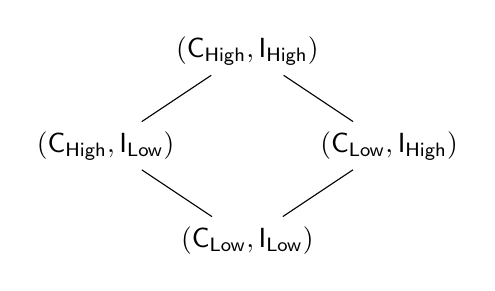
\begin{tikzpicture}[scale=1.2]
\node (HH) at (0,2) {$(\mathsf{C_{High}}, \mathsf{I_{High}})$};
\node (HL) at (-1.5,1) {$(\mathsf{C_{High}}, \mathsf{I_{Low}})$};
\node (LH) at (1.5,1) {$(\mathsf{C_{Low}}, \mathsf{I_{High}})$};
\node (LL) at (0,0) {$(\mathsf{C_{Low}}, \mathsf{I_{Low}})$};
\draw (LL) -- (HL);
\draw (LL) -- (LH);
\draw (HL) -- (HH);
\draw (LH) -- (HH);
\end{tikzpicture}
\end{center}

\textbf{Ordering}: $(c_1, i_1) \sqsubseteq (c_2, i_2)$ iff $c_1 \sqsubseteq_C c_2 \land i_2 \sqsubseteq_I i_1$

Note: Integrity is INVERTED in the product lattice.
\end{definition}

\begin{definition}[Semantic Security Under Declassification]
A program is semantically secure under a declassification policy iff for all low-equivalent initial memories, the visible outputs are equivalent:
$$M_1 \sim_L M_2 \Rightarrow \mathsf{visible}(P(M_1)) \sim_{\mathit{vis}} \mathsf{visible}(P(M_2))$$
\end{definition}

\begin{theorem}[Robustness Implies Security --- \textbf{[ChongMyers04]}, Theorem 3]
If the static robustness check passes for all declassification points, then semantic security holds.

\textbf{Robustness Condition}: For a declassification at program point $p$ with expression $e$:
\begin{enumerate}
\item $\mathsf{PC\_integrity}(p) = \mathsf{HIGH}$ (no low-integrity code on path to $p$)
\item For all $v \in \mathsf{deps}(e)$: $\mathsf{integrity}(v) = \mathsf{HIGH}$ (no low-integrity data)
\end{enumerate}
\end{theorem}

%%%%%%%%%%%%%%%%%%%%%%%%%%%%%%%%%%%%%%%%%%%%%%%%%%%%%%%%%%%%%%%%%%%%%%%%%%%%%%%
\section{Speculative Non-Interference Theorems}
\label{sec:sni}
%%%%%%%%%%%%%%%%%%%%%%%%%%%%%%%%%%%%%%%%%%%%%%%%%%%%%%%%%%%%%%%%%%%%%%%%%%%%%%%

\begin{pillarbox}[title={SPECTECTOR --- \textbf{[Guarnieri20]}}]
Speculative Non-Interference ensures that speculative execution does not reveal more than non-speculative execution.
\end{pillarbox}

\begin{definition}[SNI]
A program satisfies Speculative Non-Interference iff:
$$\forall m_1, m_2.\quad m_1 \sim_L m_2 \Rightarrow (\mathsf{trace}_{spec}(m_1) = \mathsf{trace}_{spec}(m_2) \Rightarrow \mathsf{trace}_{std}(m_1) = \mathsf{trace}_{std}(m_2))$$
\end{definition}

\begin{theorem}[Worst-Case Predictor Soundness]
SNI with worst-case predictor implies SNI with any concrete predictor.
\end{theorem}

%%%%%%%%%%%%%%%%%%%%%%%%%%%%%%%%%%%%%%%%%%%%%%%%%%%%%%%%%%%%%%%%%%%%%%%%%%%%%%%
\section{Constant-Time Product Program Theorems}
\label{sec:ct-verif}
%%%%%%%%%%%%%%%%%%%%%%%%%%%%%%%%%%%%%%%%%%%%%%%%%%%%%%%%%%%%%%%%%%%%%%%%%%%%%%%

\begin{pillarbox}[title={CT-Verif --- \textbf{[Almeida16]}}]
Constant-time security is a 2-safety hyperproperty that can be reduced to assertion checking via product program construction.
\end{pillarbox}

\begin{theorem}[Product Reduction --- \textbf{[Almeida16]}]
A program is constant-time secure iff its product program is assertion-safe:
$$\mathsf{is\_ct\_secure}(\mathit{prog}, \mathit{model}, \mathit{pub}) \iff \mathsf{is\_assertion\_safe}(\mathsf{construct\_product}(\mathit{prog}, \mathit{model}))$$

This is the main soundness theorem, verified in Coq by the CT-Verif authors.
\end{theorem}

%%%%%%%%%%%%%%%%%%%%%%%%%%%%%%%%%%%%%%%%%%%%%%%%%%%%%%%%%%%%%%%%%%%%%%%%%%%%%%%
% Cross-Reference Summary Tables
%%%%%%%%%%%%%%%%%%%%%%%%%%%%%%%%%%%%%%%%%%%%%%%%%%%%%%%%%%%%%%%%%%%%%%%%%%%%%%%

%%%%%%%%%%%%%%%%%%%%%%%%%%%%%%%%%%%%%%%%%%%%%%%%%%%%%%%%%%%%%%%%%%%%%%%%%%%%%%%
\chapter{Capability Algebra Theorems}
\label{chap:capability-algebra}
%%%%%%%%%%%%%%%%%%%%%%%%%%%%%%%%%%%%%%%%%%%%%%%%%%%%%%%%%%%%%%%%%%%%%%%%%%%%%%%

\begin{pillarbox}[title={Capability Algebra --- \textbf{[CraryWalkerMorrisett99]}}]
``Typed Memory Management''

Ownership states track LIFECYCLE (acquired $\to$ in-use $\to$ released). Multiplicities track ALIASING (unique vs potentially aliased). Both are needed for sound memory management.
\end{pillarbox}

\begin{definition}[Multiplicity Types]
\begin{itemize}
\item $\mathsf{MUnique}$: Provably no aliases exist. CAN free safely.
\item $\mathsf{MDup}$: May have aliases. Can only ACCESS, not free.
\end{itemize}
This is STRONGER than ``owned'' --- owned but aliased CANNOT free.
\end{definition}

\begin{theorem}[Free Requires Unique]
Only unique capabilities can safely free memory. This prevents use-after-free from aliased pointers.

\begin{fstarcode}[title={Free Requires Unique}]
val can_free : capability -> region -> bool
let can_free c r =
  match Map.find r c with
  | Some MUnique -> true
  | _ -> false

val free_unique_safe :
  heap:heap -> cap:capability -> r:region ->
  can_free cap r == true ->
  (forall ptr. ptr `points_to` r ==> ptr `in` cap_owned_ptrs cap r) ->
  Lemma (free heap r `results_in` safe_heap)
\end{fstarcode}
\end{theorem}

\begin{theorem}[Complete Collection --- \textbf{[Crary99]}, Section 4.2]
Well-typed terminating programs return ALL memory to the system. This proves LEAK-FREEDOM for the type system.

\begin{fstarcode}[title={Complete Collection}]
val complete_collection :
  prog:ir_program ->
  well_typed prog ->
  Lemma (
    diverges prog \/  (* Either it runs forever... *)
    (exists result. terminates prog result /\
                    final_heap prog == empty_heap)  (* ...or heap is empty *)
  )
\end{fstarcode}
\end{theorem}

%%%%%%%%%%%%%%%%%%%%%%%%%%%%%%%%%%%%%%%%%%%%%%%%%%%%%%%%%%%%%%%%%%%%%%%%%%%%%%%
\chapter{Realizability Theorems}
\label{chap:realizability}
%%%%%%%%%%%%%%%%%%%%%%%%%%%%%%%%%%%%%%%%%%%%%%%%%%%%%%%%%%%%%%%%%%%%%%%%%%%%%%%

\begin{pillarbox}[title={Realizability for Multi-Language Soundness --- \textbf{[Patterson22]}}]
``Semantic Soundness for Interoperability''

Matthews-Findler syntactic boundaries are insufficient. For SEMANTIC soundness, interpret source types as sets of TARGET values.
\end{pillarbox}

\begin{theorem}[Shared Memory Identity --- \textbf{[Patterson22]}, Section 4.2]
Sharing $\mathsf{ref}\, \tau_1$ with $\mathsf{ref}\, \tau_2$ (no copy) requires $V[\tau_1] = V[\tau_2]$.

\textbf{Examples}:
\begin{itemize}
\item Rust \texttt{\&mut i32} $\leftrightarrow$ C \texttt{int*} (same target representation)
\item Python \texttt{list} $\leftrightarrow$ C \texttt{array} (different representations, must copy)
\end{itemize}
\end{theorem}

%%%%%%%%%%%%%%%%%%%%%%%%%%%%%%%%%%%%%%%%%%%%%%%%%%%%%%%%%%%%%%%%%%%%%%%%%%%%%%%
\chapter{Verified Interpreter Pattern}
\label{chap:verified-interpreter}
%%%%%%%%%%%%%%%%%%%%%%%%%%%%%%%%%%%%%%%%%%%%%%%%%%%%%%%%%%%%%%%%%%%%%%%%%%%%%%%

\begin{pillarbox}[title={Verified Interpreter Pattern --- \textbf{[Watt18]}}]
``Mechanising and Verifying the WebAssembly Specification''

The verified interpreter pattern separates RELATIONAL specification from EXECUTABLE implementation, then proves equivalence. This provides a verified executable that is provably correct with respect to the declarative semantics.

\textbf{Key Insight}: Declarative specifications are easy to reason about but cannot execute. Executable implementations can run but are complex. By proving equivalence, we get the best of both worlds.
\end{pillarbox}

The following F* code demonstrates the core pattern: a relational reduction specification alongside an executable step function, with soundness and completeness theorems proving their equivalence.

\begin{fstarcode}[title={Verified Interpreter Core Pattern}]
module BrrrMachine.Theorems.VerifiedInterpreter

(* --------------------------------------------------
   SEPARATION OF SPECIFICATION AND IMPLEMENTATION
   Relational spec: declarative, easy to reason about
   Executable impl: can actually run, may be complex
   Prove they're equivalent -> verified executable.
   -------------------------------------------------- *)

(* Relational specification (declarative) *)
val reduce : cpg -> state -> state -> bool
(* "reduce cpg s1 s2" means s1 reduces to s2 in one step *)

(* Executable implementation (can run) *)
val step : cpg -> state -> option state
(* "step cpg s" computes next state if possible *)

(* SOUNDNESS: step produces valid reductions *)
val step_sound :
  cpg:cpg -> s:state -> s':state ->
  step cpg s = Some s' ->
  Lemma (reduce cpg s s')

(* COMPLETENESS: all reductions can be computed *)
val step_complete :
  cpg:cpg -> s:state -> s':state ->
  reduce cpg s s' ->
  Lemma (step cpg s = Some s')

(* Combined: step is a decision procedure for reduce *)
val step_decides_reduce :
  cpg:cpg -> s:state -> s':state ->
  Lemma (step cpg s = Some s' <==> reduce cpg s s')
\end{fstarcode}

The control result type below handles WebAssembly-style control flow without complex evaluation context encoding. This simplifies the interpreter while maintaining semantic precision.

\begin{fstarcode}[title={Control Result and Evaluation}]
(* --------------------------------------------------
   CONTROL RESULT TYPE
   WebAssembly-style control flow handling.
   Avoids complex evaluation context encoding.
   -------------------------------------------------- *)
type control_result =
  | Normal : state:state -> control_result
  | Break : depth:nat -> values:list value -> control_result
  | Return : values:list value -> control_result
  | Trap : reason:string -> control_result

(* Evaluation with control flow *)
val eval_with_control : cpg -> state -> control_result
let rec eval_with_control cpg state =
  match step cpg state with
  | None -> Normal state  (* Stuck = terminated *)
  | Some state' ->
      match check_control state' with
      | Some (Break d vs) -> Break d vs
      | Some (Return vs) -> Return vs
      | Some (Trap r) -> Trap r
      | None -> eval_with_control cpg state'
\end{fstarcode}

\begin{theorem}[Verified Type Checker --- \textbf{[Watt18]}, Section 4]
The same pattern applies to type checking: a relational typing judgment paired with an executable type checker, with proofs of soundness and completeness.

\begin{fstarcode}[title={Verified Type Checker}]
(* Relational typing judgment *)
val has_type : context -> expr -> ir_type -> bool

(* Executable type checker *)
val check_type : context -> expr -> option ir_type

(* Type checker soundness *)
val type_check_sound :
  ctx:context -> e:expr -> tau:ir_type ->
  check_type ctx e = Some tau ->
  Lemma (has_type ctx e tau)

(* Type checker completeness *)
val type_check_complete :
  ctx:context -> e:expr -> tau:ir_type ->
  has_type ctx e tau ->
  Lemma (check_type ctx e = Some tau)
\end{fstarcode}
\end{theorem}

\begin{pillarbox}[title={Locale-Style Abstraction for Portable Proofs}]
By abstracting over arithmetic implementation details (e.g., IEEE 754 NaN behavior), proofs work for ALL conforming implementations. This is essential for cross-platform analysis correctness.
\end{pillarbox}

\begin{fstarcode}[title={Abstract Arithmetic Interface}]
(* Abstract arithmetic interface *)
class arithmetic_impl (a : Type) = {
  add : a -> a -> a;
  mul : a -> a -> a;
  div : a -> a -> option a;  (* Partial for division by zero *)
  (* Axioms implementations must satisfy *)
  add_comm : squash (forall x y. add x y == add y x);
  add_assoc : squash (forall x y z. add (add x y) z == add x (add y z));
  (* Non-determinism specification for IEEE 754 *)
  nan_behavior : a -> bool;
}

(* Analysis sound for ALL conforming implementations *)
val analysis_sound_for_all_arith :
  #a:Type -> {| arithmetic_impl a |} ->
  cpg:cpg -> result:analysis_result ->
  result == run_analysis cpg ->
  Lemma (forall (impl : arithmetic_impl a).
    sound_wrt_impl cpg result impl)
\end{fstarcode}

%%%%%%%%%%%%%%%%%%%%%%%%%%%%%%%%%%%%%%%%%%%%%%%%%%%%%%%%%%%%%%%%%%%%%%%%%%%%%%%
\chapter{System Dependence Graph Theorems}
\label{chap:sdg}
%%%%%%%%%%%%%%%%%%%%%%%%%%%%%%%%%%%%%%%%%%%%%%%%%%%%%%%%%%%%%%%%%%%%%%%%%%%%%%%

\begin{pillarbox}[title={SDG and Two-Phase Slicing --- \textbf{[HorwitzRepsBinkley90]}}]
``Interprocedural Slicing Using Dependence Graphs''

Two-phase slicing prevents spurious interprocedural paths. Weiser's transitive closure is WRONG (context-insensitive).
\end{pillarbox}

\begin{theorem}[Two-Phase Context Sensitivity]
The two-phase algorithm produces context-sensitive slices: only nodes on REALIZABLE paths are included.

\begin{fstarcode}[title={Two-Phase Slicing}]
val interprocedural_slice : sdg -> criterion:node_id -> set node_id
let interprocedural_slice sdg crit =
  let phase1_exclude = [DefOrder; ParamOut] in
  let phase1_marked = reach_backwards sdg crit phase1_exclude in
  let phase2_exclude = [DefOrder; Call; ParamIn] in
  let phase2_marked = reach_backwards sdg phase1_marked phase2_exclude in
  Set.union phase1_marked phase2_marked

val two_phase_context_sensitive :
  sdg:sdg -> crit:node_id ->
  slice:set node_id{slice = interprocedural_slice sdg crit} ->
  Lemma (forall n. Set.mem n slice ==>
    exists path. is_realizable_path sdg path /\
                 head path = n /\ last path = crit)
\end{fstarcode}
\end{theorem}

%%%%%%%%%%%%%%%%%%%%%%%%%%%%%%%%%%%%%%%%%%%%%%%%%%%%%%%%%%%%%%%%%%%%%%%%%%%%%%%
\chapter{Probabilistic Analysis Theorems}
\label{chap:probabilistic-analysis}
%%%%%%%%%%%%%%%%%%%%%%%%%%%%%%%%%%%%%%%%%%%%%%%%%%%%%%%%%%%%%%%%%%%%%%%%%%%%%%%

\begin{pillarbox}[title={Probabilistic Abstract Interpretation --- \textbf{[CousotMonerau12]}}]
``Probabilistic Abstract Interpretation''

Probabilistic programs are measurable functions from scenario space to deterministic semantics. Classical abstract interpretation is the special case where the scenario space is a singleton. This insight enables:
\begin{itemize}
\item Branch probability estimation without profiling
\item Confidence scoring for bug reports
\item Graceful degradation from full probabilistic to non-deterministic analysis
\end{itemize}
\end{pillarbox}

The following F* code formalizes scenario spaces as probability spaces over which deterministic semantics are indexed. This generalizes classical AI where $\Omega = \{*\}$ (singleton).

\begin{fstarcode}[title={Scenario Space Abstraction}]
module BrrrMachine.Theorems.Probabilistic

(* --------------------------------------------------
   SCENARIO SPACE ABSTRACTION
   S_p[[P]] : Omega -> D
   Where:
     - Omega = probability space (scenarios)
     - D = deterministic semantics
     - mu = probability measure on Omega
   -------------------------------------------------- *)
type scenario_space (omega : Type) = {
  space : omega;
  measure : omega -> real;
  (* Measure axioms *)
  measure_positive : squash (forall s. measure s >= 0.0);
  measure_total : squash (integral measure = 1.0);
}

type prob_semantics (omega : Type) (d : Type) = {
  scenarios : scenario_space omega;
  sem : omega -> d;  (* Interpretation per scenario *)
}

(* --------------------------------------------------
   CLASSICAL AI AS SPECIAL CASE
   When Omega = {*} singleton, probabilistic AI collapses to classical AI.
   -------------------------------------------------- *)
type singleton_scenario = unit

val classical_is_singleton :
  #a:Type -> dom:abstract_domain a ->
  prob:prob_semantics singleton_scenario a ->
  prob.scenarios.space == () ->
  Lemma (prob_domain_of prob = dom)
\end{fstarcode}

Law abstraction projects to probability distributions, enabling precision-vs-cost tradeoffs. The law ordering reflects information content: more precise analyses assign higher probability to precise properties.

\begin{fstarcode}[title={Law Abstraction and Branch Probability}]
(* --------------------------------------------------
   LAW ABSTRACTION
   Abstract to probability distributions (laws).
   Law ordering reflects precision.
   -------------------------------------------------- *)
type law (a : Type) = (a -> bool) -> real  (* Pr(property holds) *)

val law_leq : #a:Type -> law a -> law a -> bool
let law_leq l1 l2 =
  (* l1 more precise than l2 if assigns higher prob to precise properties *)
  forall (q : a -> bool). l1 (downset q) >= l2 (downset q)

(* Law abstraction preserves soundness *)
val law_abstraction_sound :
  #a:Type -> {| d : abstract_domain a |} ->
  concrete_law : law a ->
  abstract_law : law a ->
  law_leq concrete_law abstract_law ->
  Lemma (forall prop. concrete_law prop >= abstract_law prop)

(* --------------------------------------------------
   BRANCH PROBABILITY ESTIMATION
   Compute branch probability from abstract domain constraints.
   No profiling needed!
   -------------------------------------------------- *)
val estimate_branch_prob :
  cpg:cpg -> cond:node_id ->
  input:abstract_state ->
  real  (* Probability condition is true *)
let estimate_branch_prob cpg cond input =
  let cond_expr = get_condition cpg cond in
  let true_states = restrict input cond_expr in
  let false_states = restrict input (negate cond_expr) in
  (* Estimate based on abstract domain volume *)
  let true_vol = volume true_states in
  let false_vol = volume false_states in
  true_vol /. (true_vol +. false_vol)
\end{fstarcode}

\begin{theorem}[Graceful Degradation]
Analysis precision can be traded for performance by merging scenarios. Soundness is preserved: degraded analysis may have less information but no false negatives for detected bugs.

\begin{fstarcode}[title={Precision Level and Degradation}]
type precision_level =
  | FullProbabilistic     (* All scenarios distinct *)
  | PartialProbabilistic  (* Some scenarios merged *)
  | NonDeterministic      (* Omega = singleton, no probability *)

val analyze_with_precision :
  cpg:cpg -> level:precision_level -> budget:duration ->
  analysis_result

(* Degradation preserves soundness *)
val degradation_sound :
  cpg:cpg ->
  full:analysis_result ->
  degraded:analysis_result ->
  full == analyze_with_precision cpg FullProbabilistic infinity ->
  degraded == analyze_with_precision cpg NonDeterministic infinity ->
  (* Degraded may have less info but no false negatives *)
  Lemma (forall bug. bug `mem` full.bugs ==> bug `mem` degraded.bugs)
\end{fstarcode}
\end{theorem}

%%%%%%%%%%%%%%%%%%%%%%%%%%%%%%%%%%%%%%%%%%%%%%%%%%%%%%%%%%%%%%%%%%%%%%%%%%%%%%%
\chapter{Unified Constraint Domain Theorems}
\label{chap:constraint-domains}
%%%%%%%%%%%%%%%%%%%%%%%%%%%%%%%%%%%%%%%%%%%%%%%%%%%%%%%%%%%%%%%%%%%%%%%%%%%%%%%

\begin{pillarbox}[title={Unified Constraint Domain --- \textbf{[XiPfenning99]}}]
``Dependent Types in Practical Programming''

All abstract domains (interval, taint, nullability, resource, ownership) share a common structure: they are instantiations of Dependent ML with different constraint systems $C$. This insight unifies:
\begin{itemize}
\item \textbf{Implementation}: One parametric domain module, many instantiations
\item \textbf{Composition}: Cross-domain reasoning via constraint conjunction
\item \textbf{Decidability}: Constraint satisfiability gives analysis termination
\item \textbf{Theory}: Single soundness proof covers all domains
\end{itemize}
\end{pillarbox}

The DML(C) pattern indexes types by constraint domain values. The following signature captures all our abstract domains uniformly.

\begin{fstarcode}[title={Unified Constraint Domain Signature}]
module BrrrMachine.Theorems.ConstraintDomains

(* --------------------------------------------------
   UNIFIED CONSTRAINT DOMAIN SIGNATURE
   Every abstract domain is an instance of this interface.
   -------------------------------------------------- *)
class constraint_domain (c : Type) = {
  (* Index sorts and terms *)
  index_sort : Type;
  index_term : Type;
  (* Constraint language *)
  constraint_ : Type;
  (* Core operations *)
  satisfiable : constraint_ -> bool;
  implies : constraint_ -> constraint_ -> bool;
  (* Abstract interpretation operations *)
  meet : constraint_ -> constraint_ -> constraint_;
  join : constraint_ -> constraint_ -> constraint_;
  widen : constraint_ -> constraint_ -> constraint_;
  (* Axioms *)
  implies_refl : squash (forall c. implies c c);
  implies_trans : squash (forall a b c. implies a b && implies b c ==> implies a c);
  meet_glb : squash (forall a b. implies (meet a b) a && implies (meet a b) b);
  join_lub : squash (forall a b. implies a (join a b) && implies b (join a b));
}
\end{fstarcode}

Each of our analysis domains becomes an instance of this unified interface:

\begin{fstarcode}[title={Domain Instantiations}]
(* Interval domain: C = linear integer arithmetic *)
instance interval_constraint_domain : constraint_domain interval = {
  index_sort = IntSort;
  index_term = LinExpr;  (* a*x + b*y + ... + c *)
  constraint_ = LinConstraint;
  satisfiable = fourier_motzkin_sat;
  implies = fun c1 c2 -> not (satisfiable (And [c1; Not c2]));
  meet = fun c1 c2 -> And [c1; c2];
  join = fun c1 c2 -> convex_hull c1 c2;
  widen = interval_widen;
}

(* Nullability domain: C = boolean constraints *)
instance null_constraint_domain : constraint_domain nullability = {
  index_sort = BoolSort;
  index_term = BoolExpr;
  constraint_ = BoolConstraint;
  satisfiable = sat_solve;
  implies = fun c1 c2 -> not (satisfiable (And [c1; Not c2]));
  meet = fun c1 c2 -> And [c1; c2];
  join = fun c1 c2 -> Or [c1; c2];
  widen = id;  (* Boolean domain is finite *)
}

(* Taint domain: C = security lattice constraints *)
instance taint_constraint_domain : constraint_domain taint = {
  index_sort = SecurityLevel;
  index_term = LevelExpr;
  constraint_ = FlowConstraint;  (* l1 <= l2 *)
  satisfiable = lattice_sat;
  implies = fun c1 c2 -> lattice_implies c1 c2;
  meet = fun c1 c2 -> And [c1; c2];
  join = fun c1 c2 -> lub_constraint c1 c2;
  widen = id;  (* Security lattice is finite *)
}
\end{fstarcode}

\begin{theorem}[Array Bounds Verification]
Using the unified constraint framework, array bounds can be statically verified via constraint solving, eliminating runtime checks when provable.

\begin{fstarcode}[title={Array Bounds Check Elimination}]
type bounds_check_result =
  | StaticallyVerified : proof:constraint_proof -> bounds_check_result
  | NeedsRuntimeCheck : bounds_check_result
  | AlwaysOutOfBounds : witness:index_term -> bounds_check_result

val check_array_bounds :
  ctx:index_constraint ->  (* What we know *)
  arr:refined_array ->
  idx:index_term ->
  bounds_check_result
let check_array_bounds ctx arr idx =
  let bounds_ok = ICAnd
    (ICPred ">=" [idx; IConst 0])
    (ICPred "<" [idx; IVar arr.length_var])
  in
  if implies ctx bounds_ok then
    StaticallyVerified (construct_proof ctx bounds_ok)
  else if satisfiable (ICAnd ctx (ICNot bounds_ok)) then
    NeedsRuntimeCheck
  else
    AlwaysOutOfBounds (find_counterexample ctx bounds_ok)

(* Bounds check elimination theorem *)
val bounds_check_elimination :
  ctx:index_constraint -> arr:refined_array -> idx:index_term ->
  check_array_bounds ctx arr idx = StaticallyVerified _ ->
  Lemma (safe_to_access arr idx)
\end{fstarcode}
\end{theorem}

\begin{theorem}[Conservative Extension --- \textbf{[XiPfenning99]}]
DML(C) is conservative over ML: existing code works unchanged. Index erasure preserves typing.

\begin{fstarcode}[title={Conservative Extension}]
(* Index erasure *)
val erase_indices : ir_refined_type -> ir_type

(* Conservative extension: typing preserved under erasure *)
val conservative_extension :
  ctx:context -> e:expr -> rt:ir_refined_type ->
  has_refined_type ctx e rt ->
  Lemma (has_type (erase_ctx ctx) (erase_expr e) (erase_indices rt))
\end{fstarcode}
\end{theorem}

%%%%%%%%%%%%%%%%%%%%%%%%%%%%%%%%%%%%%%%%%%%%%%%%%%%%%%%%%%%%%%%%%%%%%%%%%%%%%%%
\chapter{Bi-Abduction Theorems}
\label{chap:bi-abduction}
%%%%%%%%%%%%%%%%%%%%%%%%%%%%%%%%%%%%%%%%%%%%%%%%%%%%%%%%%%%%%%%%%%%%%%%%%%%%%%%

\begin{pillarbox}[title={Bi-Abduction --- \textbf{[Calcagno09]}, \textbf{[Mulder22]}}]
``Compositional Shape Analysis by means of Bi-Abduction''

Given current state $p$ and target $q$, bi-abduction discovers BOTH the missing resource $M$ (anti-frame) AND the leftover resource $F$ (frame).

Judgment: $p * ?M \vdash q * ?F$
\end{pillarbox}

\begin{theorem}[Compositionality --- \textbf{[Distefano19]}]
Analysis can be done function-by-function. Summaries capture precondition/postcondition contracts.

\begin{fstarcode}[title={Compositional Soundness}]
val compositional_soundness :
  cpg:cpg -> func:func_id -> table:map func_id procedure_summary ->
  summary:procedure_summary ->
  analyze_procedure_compositionally cpg func table = Some summary ==>
  (* For any calling context satisfying the precondition... *)
  (forall ctx. ctx `entails` summary.precondition ==>
    (* ...execution produces state satisfying postcondition *)
    exists result. executes_to cpg func ctx result /\
                   result `entails` summary.postcondition)
\end{fstarcode}
\end{theorem}

%%%%%%%%%%%%%%%%%%%%%%%%%%%%%%%%%%%%%%%%%%%%%%%%%%%%%%%%%%%%%%%%%%%%%%%%%%%%%%%
\chapter{Divergence (Non-Termination) Theorems}
\label{chap:divergence}
%%%%%%%%%%%%%%%%%%%%%%%%%%%%%%%%%%%%%%%%%%%%%%%%%%%%%%%%%%%%%%%%%%%%%%%%%%%%%%%

\begin{pillarbox}[title={Non-Termination Proving --- \textbf{[Vanegue25]}}]
``Non-Termination Proving: 100 Million LoC and Beyond''

To PROVE divergence, use UNDER-approximation. Two main detection strategies:
\begin{enumerate}
\item Repeating abstract states (loops)
\item Same-state recursive calls (recursion)
\end{enumerate}
\end{pillarbox}

\begin{theorem}[Repeating State Soundness]
A loop diverges if execution returns to the same abstract state. This is SOUND for proving divergence (under-approximation).

\begin{fstarcode}[title={Repeating State Detection}]
val repeating_state_sound :
  cpg:cpg -> w:divergence_witness{InfiniteLoop? w} ->
  Lemma (exists input. satisfies input w.path_condition /\
                       diverges (execute cpg input))
\end{fstarcode}
\end{theorem}

%%%%%%%%%%%%%%%%%%%%%%%%%%%%%%%%%%%%%%%%%%%%%%%%%%%%%%%%%%%%%%%%%%%%%%%%%%%%%%%
\chapter{Widening and Narrowing Theorems}
\label{chap:widening-narrowing}
%%%%%%%%%%%%%%%%%%%%%%%%%%%%%%%%%%%%%%%%%%%%%%%%%%%%%%%%%%%%%%%%%%%%%%%%%%%%%%%

\begin{pillarbox}[title={Widening/Narrowing --- \textbf{[Cousot92]}}]
``Comparing the Galois Connection and Widening/Narrowing Approaches''

Widening/narrowing is STRICTLY MORE POWERFUL than finite Galois connections. No finite domain can achieve equivalent results for all programs.

\textbf{Critical insight}: Discovered invariants may NOT appear in program text! Example: McCarthy's F91 $\to$ analysis discovers $[91, \mathsf{maxint}-10]$.
\end{pillarbox}

\begin{theorem}[Widening Termination]
For any ascending chain with widening, the widened chain stabilizes.

\begin{fstarcode}[title={Widening Termination}]
val widening_terminates :
  #l:lattice -> widen:widening #l -> transfer:(l.carrier -> l.carrier) ->
  Lemma (exists n.
    let rec iter k x = if k = 0 then x else iter (k-1) (widen x (transfer x)) in
    let result = iter n l.bottom in
    l.order (transfer result) result)  (* Post-fixpoint *)
\end{fstarcode}
\end{theorem}

\begin{theorem}[Narrowing Improves Precision]
\begin{fstarcode}[title={Narrowing Improvement}]
val narrowing_improves :
  #l:lattice -> narrow:narrowing #l -> transfer:(l.carrier -> l.carrier) ->
  post_widen:l.carrier ->
  l.order (transfer post_widen) post_widen ->  (* post_widen is a post-fixpoint *)
  Lemma (let refined = narrow post_widen (transfer post_widen) in
         l.order (transfer refined) refined /\  (* Still post-fixpoint *)
         l.order refined post_widen)            (* But smaller *)
\end{fstarcode}
\end{theorem}

%%%%%%%%%%%%%%%%%%%%%%%%%%%%%%%%%%%%%%%%%%%%%%%%%%%%%%%%%%%%%%%%%%%%%%%%%%%%%%%
\chapter{Symbolic Execution Theorems}
\label{chap:symbolic-execution}
%%%%%%%%%%%%%%%%%%%%%%%%%%%%%%%%%%%%%%%%%%%%%%%%%%%%%%%%%%%%%%%%%%%%%%%%%%%%%%%

\begin{pillarbox}[title={Symbolic Execution --- \textbf{[King76]}}]
``Symbolic Execution and Program Testing''

Key concepts:
\begin{enumerate}
\item Path condition (pc): Boolean expression over symbolic inputs
\item Symbolic values: Expressions over input symbols
\item Forking: When condition cannot be resolved, explore both branches
\item Commutativity: $\mathsf{instantiate}(\mathsf{exec\_symbolic}(P)) = \mathsf{exec\_concrete}(P)$
\end{enumerate}
\end{pillarbox}

\begin{theorem}[Commutativity --- \textbf{[King76]}, Section 5]
The fundamental correctness criterion for symbolic execution.

\begin{fstarcode}[title={Symbolic Execution Soundness}]
val symbolic_execution_sound :
  cpg:cpg -> func:ir_func -> tree:exec_tree -> v:valuation ->
  (* For any valuation satisfying some leaf's path condition... *)
  (exists leaf. leaf `mem` tree.leaves /\
                pc_satisfied (get_node tree leaf).state.pc v) ==>
  (* ...the symbolic result instantiated equals concrete result *)
  Lemma (
    let leaf = find_satisfied_leaf tree v in
    let sym_env = (get_node tree leaf).state.env in
    let concrete_result = execute_concrete cpg func v in
    Map.for_all (fun var sym_val ->
      instantiate sym_val v = Map.find var concrete_result
    ) sym_env)
\end{fstarcode}
\end{theorem}

%%%%%%%%%%%%%%%%%%%%%%%%%%%%%%%%%%%%%%%%%%%%%%%%%%%%%%%%%%%%%%%%%%%%%%%%%%%%%%%
\chapter{Frame Rule and Local Reasoning}
\label{chap:frame-rule}
%%%%%%%%%%%%%%%%%%%%%%%%%%%%%%%%%%%%%%%%%%%%%%%%%%%%%%%%%%%%%%%%%%%%%%%%%%%%%%%

\begin{pillarbox}[title={Separation Logic Frame Rule --- \textbf{[Reynolds02]}}]
``Separation Logic: A Logic for Shared Mutable Data Structures''

The Frame Rule enables COMPOSITIONAL analysis by allowing us to reason about a command using only its ``footprint'' (accessed memory).
\end{pillarbox}

\begin{theorem}[Frame Rule --- \textbf{[Reynolds02]}, Theorem 1]
$$\frac{\{p\}\, c\, \{q\}}{\{p * r\}\, c\, \{q * r\}}$$

\textbf{Side condition}: $r$ does not mention modified variables or freed locations.

\begin{fstarcode}[title={Frame Rule}]
val frame_rule :
  p:sl_assertion -> c:ir_stmt -> q:sl_assertion ->
  r:sl_assertion ->
  hoare_valid p c q ->
  disjoint (footprint c).writes (free_vars r) ->
  disjoint (footprint c).frees (locs_in r) ->
  Lemma (hoare_valid (SLSep p r) c (SLSep q r))
\end{fstarcode}
\end{theorem}

\begin{theorem}[Parallel Rule --- \textbf{[Reynolds02]}, Section 11.3]
$$\frac{\{p_1\}\, c_1\, \{q_1\} \quad \{p_2\}\, c_2\, \{q_2\}}{\{p_1 * p_2\}\, c_1 \parallel c_2\, \{q_1 * q_2\}}$$

\textbf{Side condition}: Disjoint footprints.

\textbf{Corollary}: Disjoint parallel threads do not race.
\end{theorem}

%%%%%%%%%%%%%%%%%%%%%%%%%%%%%%%%%%%%%%%%%%%%%%%%%%%%%%%%%%%%%%%%%%%%%%%%%%%%%%%
\chapter{Effect Handler Correctness Theorems}
\label{chap:effect-handlers}
%%%%%%%%%%%%%%%%%%%%%%%%%%%%%%%%%%%%%%%%%%%%%%%%%%%%%%%%%%%%%%%%%%%%%%%%%%%%%%%

\begin{pillarbox}[title={Algebraic Effects --- \textbf{[PlotkinPretnar09]}}]
``Handlers of Algebraic Effects''

Key insight: Handlers are HOMOMORPHISMS from free algebraic models. A handler is CORRECT if it forms a valid model of the effect theory.

\textbf{CRITICAL LIMITATIONS}:
\begin{itemize}
\item Continuations (call/cc) are NOT algebraic effects
\item Parallel composition CANNOT be expressed with unary handlers
\end{itemize}
\end{pillarbox}

\begin{fstarcode}[title={Effect Signature and Handler}]
module BrrrMachine.EffectHandlers

type operation = {
  name : string;
  param_type : Type;
  arity : nat;
  result_types : list Type;
}

type effect_signature = {
  operations : list operation;
  equations : list effect_equation;
}

type handler (e:effect_signature) (m:Type) = {
  handle_return : value -> m;
  handle_op : op:operation{op `mem` e.operations} ->
              op.param_type ->
              (op.result_types -> m) ->
              m;
}
\end{fstarcode}

\begin{theorem}[Handler Correctness --- \textbf{[PlotkinPretnar09]}]
A handler is CORRECT if it preserves the effect theory's equations.

\begin{fstarcode}[title={Handler Correctness}]
val handler_correct :
  #e:effect_signature -> #m:Type -> h:handler e m ->
  (* Handler must preserve all equations *)
  (forall eq. eq `mem` e.equations ==>
    interpret_with_handler h eq.lhs == interpret_with_handler h eq.rhs)
\end{fstarcode}
\end{theorem}

%%%%%%%%%%%%%%%%%%%%%%%%%%%%%%%%%%%%%%%%%%%%%%%%%%%%%%%%%%%%%%%%%%%%%%%%%%%%%%%
\chapter{Probabilistic Semantics Theorems}
\label{chap:probabilistic-semantics}
%%%%%%%%%%%%%%%%%%%%%%%%%%%%%%%%%%%%%%%%%%%%%%%%%%%%%%%%%%%%%%%%%%%%%%%%%%%%%%%

\begin{pillarbox}[title={Probabilistic Programs --- \textbf{[Kozen81]}}]
``Semantics of Probabilistic Programs''

Key insight: Programs are LINEAR OPERATORS on MEASURES. Dual semantics:
\begin{enumerate}
\item Operational: $f_S : X^{n+\omega} \to X^{n+\omega}$ (input with random tape $\to$ output)
\item Denotational: $S : B \to B$ (input distribution $\to$ output distribution)
\end{enumerate}
\end{pillarbox}

\begin{theorem}[Discrete Sufficiency --- \textbf{[Kozen81]}, Theorem 6.1]
If two programs agree on all point masses, they agree on all distributions.

\begin{fstarcode}[title={Discrete Sufficiency}]
val discrete_sufficiency :
  s1:(state -> linear_operator state) ->
  s2:(state -> linear_operator state) ->
  (* If they agree on all point masses... *)
  (forall x. s1 (point_mass x) == s2 (point_mass x)) ==>
  (* ...they agree on all distributions *)
  Lemma (forall mu. s1 mu == s2 mu)
\end{fstarcode}

\textbf{Application}: Testing on discrete inputs is SUFFICIENT for correctness validation.
\end{theorem}

%%%%%%%%%%%%%%%%%%%%%%%%%%%%%%%%%%%%%%%%%%%%%%%%%%%%%%%%%%%%%%%%%%%%%%%%%%%%%%%
\chapter{Set Constraint Resolution Theorems}
\label{chap:set-constraints}
%%%%%%%%%%%%%%%%%%%%%%%%%%%%%%%%%%%%%%%%%%%%%%%%%%%%%%%%%%%%%%%%%%%%%%%%%%%%%%%

\begin{pillarbox}[title={Set Constraints --- \textbf{[Aiken99]}}]
``Introduction to Set Constraint-Based Program Analysis''

Key insight: Dataflow, type inference, and closure analysis are ALL instances of set constraint solving. Constraint form:
$$E_1 \subseteq E_2 \quad\text{where}\quad E ::= \alpha \mid \emptyset \mid E_1 \cup E_2 \mid E_1 \cap E_2 \mid \neg E \mid c(E_1,\ldots,E_n) \mid c^{-i}(E) \mid Y \Rightarrow X$$
\end{pillarbox}

\begin{theorem}[Inductive Form Existence --- \textbf{[Aiken99]}, Section 5]
Any satisfiable constraint system can be transformed to inductive form with finite representation.

\begin{fstarcode}[title={Inductive Form}]
val inductive_form_theorem :
  cs:constraint_system ->
  Lemma (satisfiable cs <==>
         exists (sys:inductive_system).
           forall sol. satisfies_all sol cs <==>
                       exists beta. sol = extract_solution sys beta)
\end{fstarcode}
\end{theorem}

\begin{theorem}[Function Subtyping (Contravariance)]
$$(\tau_1 \to \tau_2) \subseteq (\sigma_1 \to \sigma_2) \iff \sigma_1 \subseteq \tau_1 \land \tau_2 \subseteq \sigma_2$$

Note: Domain is CONTRAVARIANT, codomain is covariant.
\end{theorem}

%%%%%%%%%%%%%%%%%%%%%%%%%%%%%%%%%%%%%%%%%%%%%%%%%%%%%%%%%%%%%%%%%%%%%%%%%%%%%%%
\chapter{Datalog Compilation and Analysis Composition}
\label{chap:datalog-compilation}
%%%%%%%%%%%%%%%%%%%%%%%%%%%%%%%%%%%%%%%%%%%%%%%%%%%%%%%%%%%%%%%%%%%%%%%%%%%%%%%

\begin{pillarbox}[title={Datalog Compilation --- \textbf{[Jordan16]}, \textbf{[Madsen16]}}]
``Souffle: On Synthesis of Program Analyzers'' and ``From Datalog to Flix''

\textbf{Key Insight}: COMPILE Datalog rules to specialized code, don't interpret them. Compilation achieves 50x+ speedup over interpretation (bddbddb, muZ).

\textbf{Benchmark} (OpenJDK7: 1.4M variables, 350K objects, 160K methods):\\
Souffle (compiled): 35 seconds | bddbddb: 30 minutes | SQLite: 6h20m | muZ: DNF
\end{pillarbox}

The Souffle compilation pipeline uses staged specialization via Futamura projections. Each stage eliminates interpretation overhead while preserving semantics.

\begin{fstarcode}[title={Datalog Compilation Pipeline}]
module BrrrMachine.DatalogCompile

(* --------------------------------------------------
   RELATIONAL ALGEBRA MACHINE (RAM) OPERATIONS
   Source: Jordan, Scholz, Subotic 2016
   RAM is the intermediate representation between Datalog rules and
   generated code. Enables optimization before code generation.
   -------------------------------------------------- *)
type ram_expr =
  | RAMScan : relation:string -> ram_expr
  | RAMFilter : expr:ram_expr -> column:nat -> value:string -> ram_expr
  | RAMProject : expr:ram_expr -> columns:list nat -> ram_expr
  | RAMJoin : left:ram_expr -> right:ram_expr ->
              left_col:nat -> right_col:nat -> ram_expr
  | RAMUnion : left:ram_expr -> right:ram_expr -> ram_expr
  | RAMDiff : left:ram_expr -> right:ram_expr -> ram_expr

type ram_stmt =
  | RAMInsert : target:string -> source:ram_expr -> ram_stmt
  | RAMLoop : delta:string -> body:list ram_stmt -> ram_stmt  (* Semi-naive *)
  | RAMSeq : stmts:list ram_stmt -> ram_stmt
\end{fstarcode}

\begin{theorem}[Optimal Index Selection via Dilworth's Theorem --- \textbf{[Jordan16]}]
Given $N$ index requirements from queries, find MINIMAL set of indices such that each requirement is subsumed by at least one selected index.

\textbf{Insight}: Index subsumption forms a partial order. A lexicographic index $[a, b, c]$ subsumes $[a, b]$ and $[a]$. Dilworth's theorem: the width of a partial order equals the minimum number of chains needed to cover all elements.

\begin{fstarcode}[title={Dilworth-Based Index Selection}]
(* Index specification *)
type index_spec = {
  relation : string;
  key_columns : list nat;  (* Lexicographic order *)
}

(* Index subsumption: [a,b,c] subsumes [a,b] and [a] *)
let subsumes (super sub : index_spec) : bool =
  super.relation = sub.relation &&
  List.length sub.key_columns <= List.length super.key_columns &&
  List.for_all2 (=) sub.key_columns
    (List.take (List.length sub.key_columns) super.key_columns)

(* Dilworth-based minimal index selection *)
val compute_minimal_indices :
  required:list index_spec ->
  minimal:list index_spec{
    (* Every required index is subsumed by some minimal index *)
    forall r. List.mem r required ==>
      exists m. List.mem m minimal /\ subsumes m r
  }
\end{fstarcode}
\end{theorem}

\begin{pillarbox}[title={Lattice-Extended Datalog --- \textbf{[Madsen16]}}]
Standard Datalog operates on relations (finite sets). Flix extends Datalog with lattice predicates, enabling elegant expression of IFDS, IDE, and value analyses.

\textbf{Key Difference}:
\begin{itemize}
\item Standard Datalog: Multiple tuples with same key = set (keep all)
\item Flix Extension: Same key = JOIN lattice values (collapse to single)
\end{itemize}

This enables constant propagation, interval analysis, and IDE (micro-function lattices).
\end{pillarbox}

The following F* code shows how IDE is expressed as Flix with a specific lattice: the micro-function space of environment transformers.

\begin{fstarcode}[title={IDE as Lattice-Extended Datalog}]
module BrrrMachine.IDE

(* --------------------------------------------------
   IDE IS FLIX WITH MICRO-FUNCTION LATTICE
   Source: Madsen, Yee, Lhotak 2016

   IFDS path edge:  PathEdge(d1, n, d2)           -- fact d2 holds at n
   IDE path edge:   PathEdge(d1, n, d2, f)        -- with environment xformer
                                       ^^
                              micro-function lattice element

   IDE key insight: transformers COMPOSE along paths
     PathEdge(d1, m, d3, compose(f, g)) :-
       PathEdge(d1, n, d2, f),
       CFG(n, m),
       EdgeFunction(n, d2, m, d3, g).
   -------------------------------------------------- *)

(* Micro-function: environment transformer *)
type micro_fn (v : Type) = v -> v

(* Micro-functions form a lattice under pointwise ordering *)
instance micro_fn_lattice (v : Type) {| complete_lattice v |} :
  complete_lattice (micro_fn v) = {
  bot = (fun _ -> bot);
  top = (fun _ -> top);
  join = (fun f g -> fun x -> join (f x) (g x));
  meet = (fun f g -> fun x -> meet (f x) (g x));
  leq = (fun f g -> forall x. leq (f x) (g x));
}

(* Micro-function composition for IDE path edges *)
val compose_micro : #v:Type -> {| complete_lattice v |} ->
                    micro_fn v -> micro_fn v -> micro_fn v
let compose_micro f g = fun x -> f (g x)

(* Distributivity requirement for IFDS/IDE soundness *)
val distributive_transfer :
  #d:Type -> {| complete_lattice d |} ->
  f:micro_fn d ->
  Lemma (requires forall x y. f (join x y) == join (f x) (f y))
        (ensures distributive f)
\end{fstarcode}

\begin{theorem}[Semantic Preservation --- \textbf{[Jordan16]}]
The staged translation preserves Datalog semantics:
$$\mathsf{result} = \llbracket \mathsf{Int} \rrbracket(\mathsf{Source}, \mathsf{Input}) = \llbracket \mathsf{Compiled} \rrbracket(\mathsf{Input})$$

\begin{fstarcode}[title={Compilation Correctness}]
(* Compilation correctness theorem *)
val compilation_correct :
  prog:datalog_program ->
  Lemma (eval_compiled (compile_to_ram prog) == datalog_semantics prog)

(* IFDS can be expressed as Datalog for compilation *)
val ifds_to_datalog : #d:Type -> ifds_problem d -> datalog_program

(* Compiled IFDS computes same result as tabulation algorithm *)
val compiled_ifds_correct : #d:Type ->
  prob:ifds_problem d ->
  Lemma (eval_compiled (compile_ifds prob) == ifds_tabulation prob)
\end{fstarcode}
\end{theorem}

%%%%%%%%%%%%%%%%%%%%%%%%%%%%%%%%%%%%%%%%%%%%%%%%%%%%%%%%%%%%%%%%%%%%%%%%%%%%%%%
\chapter{Local-to-Global Consistency Theorems}
\label{chap:local-global}
%%%%%%%%%%%%%%%%%%%%%%%%%%%%%%%%%%%%%%%%%%%%%%%%%%%%%%%%%%%%%%%%%%%%%%%%%%%%%%%

\begin{pillarbox}[title={Local-Global Consistency --- \textbf{[Cousot77]}}]
``Abstract Interpretation: A Unified Lattice Model''

Key insight: If abstract interpretation is locally consistent with concrete semantics, then global analysis results are sound. This enables MODULAR soundness proofs.
\end{pillarbox}

\begin{theorem}[Fundamental Theorem of Abstract Interpretation --- \textbf{[Cousot77]}, Theorem 4.1]
Local consistency implies global consistency.

\begin{fstarcode}[title={Local-Global Consistency}]
val local_global_consistency :
  #c:Type -> #a:Type ->
  gc:galois_connection c a ->
  f_c:(c -> c) -> f_a:(a -> a) ->
  locally_consistent gc f_c f_a ->
  monotone f_c -> monotone f_a ->
  Lemma (forall n.
    gc.alpha (iterate f_c n gc.concrete_lattice.bot) `leq_a`
    iterate f_a n gc.abstract_lattice.bot)

(* Corollary: Fixpoints are consistent *)
val fixpoint_consistency :
  #c #a gc f_c f_a ->
  locally_consistent gc f_c f_a ->
  monotone f_c -> monotone f_a ->
  Lemma (gc.alpha (lfp f_c) `leq_a` lfp f_a)
\end{fstarcode}
\end{theorem}

%%%%%%%%%%%%%%%%%%%%%%%%%%%%%%%%%%%%%%%%%%%%%%%%%%%%%%%%%%%%%%%%%%%%%%%%%%%%%%%
\chapter{Boundary Guard Soundness Theorems}
\label{chap:boundary-guards}
%%%%%%%%%%%%%%%%%%%%%%%%%%%%%%%%%%%%%%%%%%%%%%%%%%%%%%%%%%%%%%%%%%%%%%%%%%%%%%%

\begin{pillarbox}[title={Boundary Guards --- \textbf{[MatthewsFindler07]}}]
``Operational Semantics for Multi-Language Programs''

Boundaries between languages require GUARDS to ensure type safety. Guards have POLARITY that flips at function types.
\end{pillarbox}

\begin{definition}[Guard Polarity]
\begin{itemize}
\item \textbf{Positive}: Value entering STRICTER language (dynamic $\to$ static). MUST check.
\item \textbf{Negative}: Value from STRICTER language (static $\to$ dynamic). Can skip.
\end{itemize}
\end{definition}

\begin{theorem}[Guard Soundness --- \textbf{[MatthewsFindler07]}, Theorem 1]
Guards ensure type soundness at boundaries.

\begin{fstarcode}[title={Guard Soundness}]
val guard_soundness :
  source:language_config ->
  target:language_config ->
  e:expr -> ty:ir_type ->
  pol:guard_polarity{pol = polarity source target} ->
  guard:guard{guard = generate_guard ty pol} ->
  well_typed source e ty ->
  Lemma (reduces_safely target (apply_guard guard (eval source e)))
\end{fstarcode}
\end{theorem}

\begin{theorem}[Lump Cancellation]
Boundary pairs cancel: $\hat{\tau}\, \mathsf{MS}(\mathsf{SM}\, \hat{\tau}\, v) \to v$

\begin{fstarcode}[title={Cancellation}]
val cancellation_sound :
  e:boundary_expr ->
  Lemma (eval_boundary e = eval_boundary (cancel_boundaries e))
\end{fstarcode}
\end{theorem}

%%%%%%%%%%%%%%%%%%%%%%%%%%%%%%%%%%%%%%%%%%%%%%%%%%%%%%%%%%%%%%%%%%%%%%%%%%%%%%%
\chapter{Vault Adoption and Focus Theorems}
\label{chap:vault}
%%%%%%%%%%%%%%%%%%%%%%%%%%%%%%%%%%%%%%%%%%%%%%%%%%%%%%%%%%%%%%%%%%%%%%%%%%%%%%%

\begin{pillarbox}[title={Vault --- \textbf{[DeLine01]}, \textbf{[DeLine02]}, \textbf{[DeLine04]}}]
``Vault, Fugue: Typestate for Object-Oriented Languages''

Adoption permanently transfers unique ownership to shared-frozen state. Focus temporarily upgrades shared permission to unique within a scope.
\end{pillarbox}

\begin{theorem}[Adoption Preserves Typestate]
Adoption is irreversible and freezes typestate.

\begin{fstarcode}[title={Adoption Soundness}]
val adoption_preserves_typestate :
  perm:access_permission_v2{APUnique_v2? perm} ->
  state_at_adoption:state_node ->
  Lemma (let (APUnique_v2 r n g) = perm in
         let adopted = APPure_v2 r n g (Some n) in
         n = state_at_adoption ==>
         forever_frozen adopted n)

val adoption_irreversible :
  original:access_permission_v2{APUnique_v2? original} ->
  Lemma (let adopted = perform_adoption original in
         APPure_v2? adopted /\
         not (exists op. apply_transition adopted op = Some (APUnique_v2? _)))
\end{fstarcode}
\end{theorem}

\begin{theorem}[Focus Scope Soundness]
Focus temporarily upgrades shared to unique, with proper scope management.

\begin{fstarcode}[title={Focus Soundness}]
val focus_scope_sound :
  original:access_permission_v2{APPure_v2? original} ->
  lock_acquired:bool ->
  body:(access_permission_v2 -> access_permission_v2) ->
  (FocusSuccess? (enter_focus original lock_acquired)) ==>
  Lemma (let FocusSuccess token unique = enter_focus original lock_acquired in
         let result = body unique in
         let restored = exit_focus token result in
         APPure_v2? restored /\
         get_state restored = get_state result)
\end{fstarcode}
\end{theorem}

%%%%%%%%%%%%%%%%%%%%%%%%%%%%%%%%%%%%%%%%%%%%%%%%%%%%%%%%%%%%%%%%%%%%%%%%%%%%%%%
\chapter{Stack Filtering Theorems (Rupta)}
\label{chap:stack-filtering}
%%%%%%%%%%%%%%%%%%%%%%%%%%%%%%%%%%%%%%%%%%%%%%%%%%%%%%%%%%%%%%%%%%%%%%%%%%%%%%%

\begin{pillarbox}[title={Stack Filtering --- \textbf{[Li24]}}]
``Rupta: Efficient and Precise Pointer Analysis for Rust''

\textbf{NOTE}: This is a NOVEL technique not found in prior literature.

Stack objects allocated in function $f$ are ONLY alive when $f$'s frame is on the call stack. Filtering out dead stack objects dramatically improves both PRECISION and SPEED.
\end{pillarbox}

\begin{theorem}[Stack Filtering Soundness]
If we filter out a stack location from a points-to set, then that location cannot be pointed to in any concrete execution at that program point.

\begin{fstarcode}[title={Stack Filtering Soundness}]
val stack_filtering_sound :
  cg:call_graph -> pts:pts_solution ->
  var:var_id -> ctx:context ->
  filtered:set abstract_loc{filtered = filter_dead_stack cg pts var ctx} ->
  Lemma (forall loc. loc `in` filtered ==>
    loc `in` concrete_pts var ctx)
\end{fstarcode}
\end{theorem}

%%%%%%%%%%%%%%%%%%%%%%%%%%%%%%%%%%%%%%%%%%%%%%%%%%%%%%%%%%%%%%%%%%%%%%%%%%%%%%%
% Cross-Reference Summary Tables
%%%%%%%%%%%%%%%%%%%%%%%%%%%%%%%%%%%%%%%%%%%%%%%%%%%%%%%%%%%%%%%%%%%%%%%%%%%%%%%

\begin{table}[htbp]
\centering
\caption{Part XII Theorem Cross-References}
\label{tab:part12-crossref}
\begin{tabular}{@{}lll@{}}
\toprule
\textbf{Theorem} & \textbf{Source} & \textbf{Related Sections} \\
\midrule
Abstract Interpretation Soundness & \textbf{[Cousot77]} & Section 2.1 \\
IFDS Soundness/Completeness & \textbf{[Reps95]} & Section 4.1 \\
True Positives Property & \textbf{[Le22]} & Section 12.3 \\
Occurrence Typing Soundness & \textbf{[TobinHochstadt08]} & Section 2.1.7b \\
DRF-SC Theorem & \textbf{[Batty11]} & Section 6.5 \\
Effect Absence Theorems & \textbf{[Leijen14]} & Section 6.1.3 \\
Session Type Safety & \textbf{[Honda08]} & Section 7.3 \\
SVF Soundness & \textbf{[Sui12]} & Section 5.6 \\
ZIPPER Precision & \textbf{[Li20]} & Section 5.3.2 \\
CSE Soundness & \textbf{[Trabish18]} & Section 4.4.6 \\
FTG Soundness & \textbf{[Huang23]} & Section 5.3.3 \\
DSA Soundness & \textbf{[Lattner07]} & Section 5.2.5 \\
Robustness Theorem & \textbf{[ChongMyers04]} & Section 8.1.4.3 \\
SNI Soundness & \textbf{[Guarnieri20]} & Section 8.1.4.6 \\
CT-Verif Reduction & \textbf{[Almeida16]} & Section 8.1.4.7 \\
Capability Algebra & \textbf{[CraryWalkerMorrisett99]} & Section 7.1 \\
Realizability & \textbf{[Patterson22]} & Section 9.1 \\
SDG Two-Phase & \textbf{[HorwitzRepsBinkley90]} & Section 3.3 \\
Bi-Abduction & \textbf{[Calcagno09]} & Section 7.4 \\
Divergence Analysis & \textbf{[Vanegue25]} & Section 4.4 \\
Widening/Narrowing & \textbf{[Cousot92]} & Section 2.3 \\
Symbolic Execution & \textbf{[King76]} & Section 4.4 \\
Frame Rule & \textbf{[Reynolds02]} & Section 7.4 \\
Stack Filtering & \textbf{[Li24]} & Section 5.3.4 \\
\bottomrule
\end{tabular}
\end{table}

%%%%%%%%%%%%%%%%%%%%%%%%%%%%%%%%%%%%%%%%%%%%%%%%%%%%%%%%%%%%%%%%%%%%%%%%%%%%%%%
% Extended Cross-Reference Summary
%%%%%%%%%%%%%%%%%%%%%%%%%%%%%%%%%%%%%%%%%%%%%%%%%%%%%%%%%%%%%%%%%%%%%%%%%%%%%%%

\begin{table}[htbp]
\centering
\caption{Part XII Section Summary}
\label{tab:part12-sections}
\begin{tabular}{@{}llp{6cm}@{}}
\toprule
\textbf{Section} & \textbf{Topic} & \textbf{Key Theorems} \\
\midrule
12.1 & Module Structure & F* module hierarchy \\
12.2 & Soundness Theorems & AI, IFDS, Taint, Boundary, Ownership \\
12.3 & Manifest/Latent & True Positives Property, Falsification \\
12.4 & Under-Approximation & Reversed Consequence, Disjunction \\
12.5 & Manifest Errors & Outcome Logic characterization \\
12.6 & Capability Algebra & Free Requires Unique, Complete Collection \\
12.7 & Realizability & Shared Memory Identity \\
12.8 & Verified Interpreter & Specification-Implementation equivalence \\
12.9 & SDG Theorems & Two-Phase slicing \\
12.10 & Probabilistic & Scenario space, Law abstraction \\
12.11 & Constraint Domains & DML(C) unification \\
12.12 & Bi-Abduction & Compositional analysis \\
12.13 & Divergence & Repeating states, Recursive divergence \\
12.14 & Widening/Narrowing & Termination, Precision improvement \\
12.15 & Symbolic Execution & Commutativity theorem \\
12.16 & Effect Handlers & Algebraic effect correctness \\
12.17 & Probabilistic Semantics & Linear operators on measures \\
12.18 & Set Constraints & Resolution complexity \\
12.19 & Local-Global Consistency & Fundamental AI theorem \\
12.20 & Boundary Guards & Guard soundness \\
12.21 & Frame Rule & Separation logic compositionality \\
12.22 & Stack Filtering & Rupta precision theorem \\
12.25 & Institution Theory & Satisfaction condition \\
12.26 & C11 Memory Model & DRF-SC theorem \\
12.27 & Effect Absence & Exception, Termination, State isolation \\
12.28 & Session Types & Communication safety, Fidelity, Progress \\
12.29 & SVF Theorems & Memory SSA, SVFG, Leak detection \\
12.30 & ZIPPER & PFG captures flows, Precision preservation \\
12.31 & Chopped SE & Soundness, Relative completeness \\
12.32 & Python FTG & Type safety, Call graph soundness \\
12.33 & DSA Theorems & Completeness, Soundness, Heap cloning \\
12.34 & Robust Declassification & Robustness implies security, SNI, CT-Verif \\
\bottomrule
\end{tabular}
\end{table}
